% Chapter Template

\chapter{Agile using Scrum} % Main chapter title

\label{Chapter_Agile_and_Scrum} % Change X to a consecutive number; for referencing this chapter elsewhere, use \ref{ChapterX}

%----------------------------------------------------------------------------------------

\section{Overview}

The Manifesto for Agile Software Development sets out the overarching principles
of agile software development \parencite{Beck2001ManifestoFA}:

\begin{displayquote}
``We are uncovering better ways of developing software by doing it and helping 
others do it. Through this work we have come to value:

\begin{itemize}
	\item \textbf{Individuals and interactions} \textit{over} processes and tools 
	\item \textbf{Working software} \textit{over} comprehensive documentation 
	\item \textbf{Customer collaboration} \textit{over} contract negotiation 
	\item \textbf{Responding to change} \textit{over} following a plan 
\end{itemize}

That is, while there is value in the items on the right, we value the items on
the left more.''
\end{displayquote}

This is further expanded on by the Twelve Principles of Agile Software
\parencite{Beck2001ManifestoFA}:

\begin{displayquote}
``We follow these principles:

\begin{enumerate}
	\item Our highest priority is to satisfy the customer
		through early and continuous delivery
		of valuable software.

	\item Welcome changing requirements, even late in
		development. Agile processes harness change for
		the customer's competitive advantage.

	\item Deliver working software frequently, from a
		couple of weeks to a couple of months, with a
		preference to the shorter timescale.

	\item Business people and developers must work
		together daily throughout the project.

	\item Build projects around motivated individuals.
		Give them the environment and support they need,
		and trust them to get the job done.

	\item The most efficient and effective method of
		conveying information to and within a development
		team is face-to-face conversation.

	\item Working software is the primary measure of progress.

	\item Agile processes promote sustainable development.
		The sponsors, developers, and users should be able
		to maintain a constant pace indefinitely.

	\item Continuous attention to technical excellence
		and good design enhances agility.

	\item Simplicity--the art of maximizing the amount
		of work not done--is essential.

	\item The best architectures, requirements, and designs
		emerge from self-organizing teams.

	\item At regular intervals, the team reflects on how
		to become more effective, then tunes and adjusts
		its behaviour accordingly.''
\end{enumerate}

\end{displayquote}

Scrum is an agile project management methodology. It focuses on short feedback
loops. Scrum is described in terms of roles, events, and artefacts. The Scrum 
process workflow is shown in Figure \ref{fig:ScrumWorkflow}.

\section{Scrum roles}
The scrum team consists of a Product Owner, the Development Team, and a Scrum Master.
The scrum team is self-organizing and cross-functional. The Scrum team has all the skills 
necessary to complete assigned tasks without outside assistance \parencite{TheScrumGuide}.

\subsection{Product Owner}
The Product Owner is one person. The Product Owner may represent a committee of people, 
but the Product Owner must only be one person. The Product Owner is responsible 
for maximizing the value of the product resulting from the work done by the 
Development Team. The product owner is the only one responsible for managing the
Product Backlog. The rest of the team may help manage the backlog but the 
Product Owner is the only accountable person  \parencite{TheScrumGuide}.

\subsection{Development Team}
The Development Team is a small team consisting of between three and nine 
professional people. The Development Team members do the work necessary to 
deliver a potentially releasable increment of the product. A completed potentially
releasable increment of the product is required at the Sprint Review  \parencite{TheScrumGuide}.

\subsection{Scrum Master}
The Scrum Master is the servant-leader of the Scrum Team. The Scrum Master 
facilitates the interaction between outsiders and the team. The Scrum Master steers 
the interaction between team members to maximize the value create by the 
Scrum Team  \parencite{TheScrumGuide}.

\section{Scrum Events}
Scrum Events are used the create a regular rhythm and minimizes the need for 
irregular disrupting causing meetings \parencite{TheScrumGuide}.

\subsection{Sprint}
The Sprint is the core of Scrum. A Sprint is a period, no longer than a month, in which 
a usable and potentially releasable increment of the product is created. The length
of the Sprint does not change throughout the development process. The next Sprint 
starts directly after the previous Sprint finishes. The Sprint contains and consists of the 
Sprint Planning, Daily Scrum, the development work, the Sprint Review, and the 
Sprint Retrospective \parencite{TheScrumGuide}.

\subsection{Daily Scrum}
The Daily Scrum is a 15 minute event for the Development Team. During the Daily 
Scrum the Development Team plans the work for the next 24 hours that is needed
to achieve the Sprint Goal  \parencite{TheScrumGuide}.

\subsection{Sprint Review}
A Sprint Review is held at the end of the Sprint to inspect the Product Increment 
and adapt the Product Backlog  \parencite{TheScrumGuide}.

\subsection{Sprint Retrospective}
The Sprint Retrospective is held at the end of the Sprint to allow the Scrum Team
an opportunity for introspection to plan for improvements that can be 
done in the next Sprint  \parencite{TheScrumGuide}.

\section{Scrum Artefacts}
Scrum Artifacts represent work done or provide information about the development 
process in order to provide transparency \parencite{TheScrumGuide}.

\subsection{Product Backlog}
The Product Backlog is an ordered list of every known requirement of the product.
The Product Backlog is always evolving as new requirement are discovered. It is 
the only source of required changes to the product. The Product owner is 
responsible for the Product Backlog, this includes its content, availability, 
and ordering \parencite{TheScrumGuide}.

\subsection{Sprint Backlog}
The Sprint Backlog is the set of Product Backlog items selected for the Sprint
and a plan for delivering the product Increment, realizing the Sprint Goal \parencite{TheScrumGuide}.

\subsection{Increment}
The Increment is the sum of all the Product Backlog items completed during a 
Sprint and the value of the increments of all previous Sprints \parencite{TheScrumGuide}.

\begin{figure}[H]
	\centering
	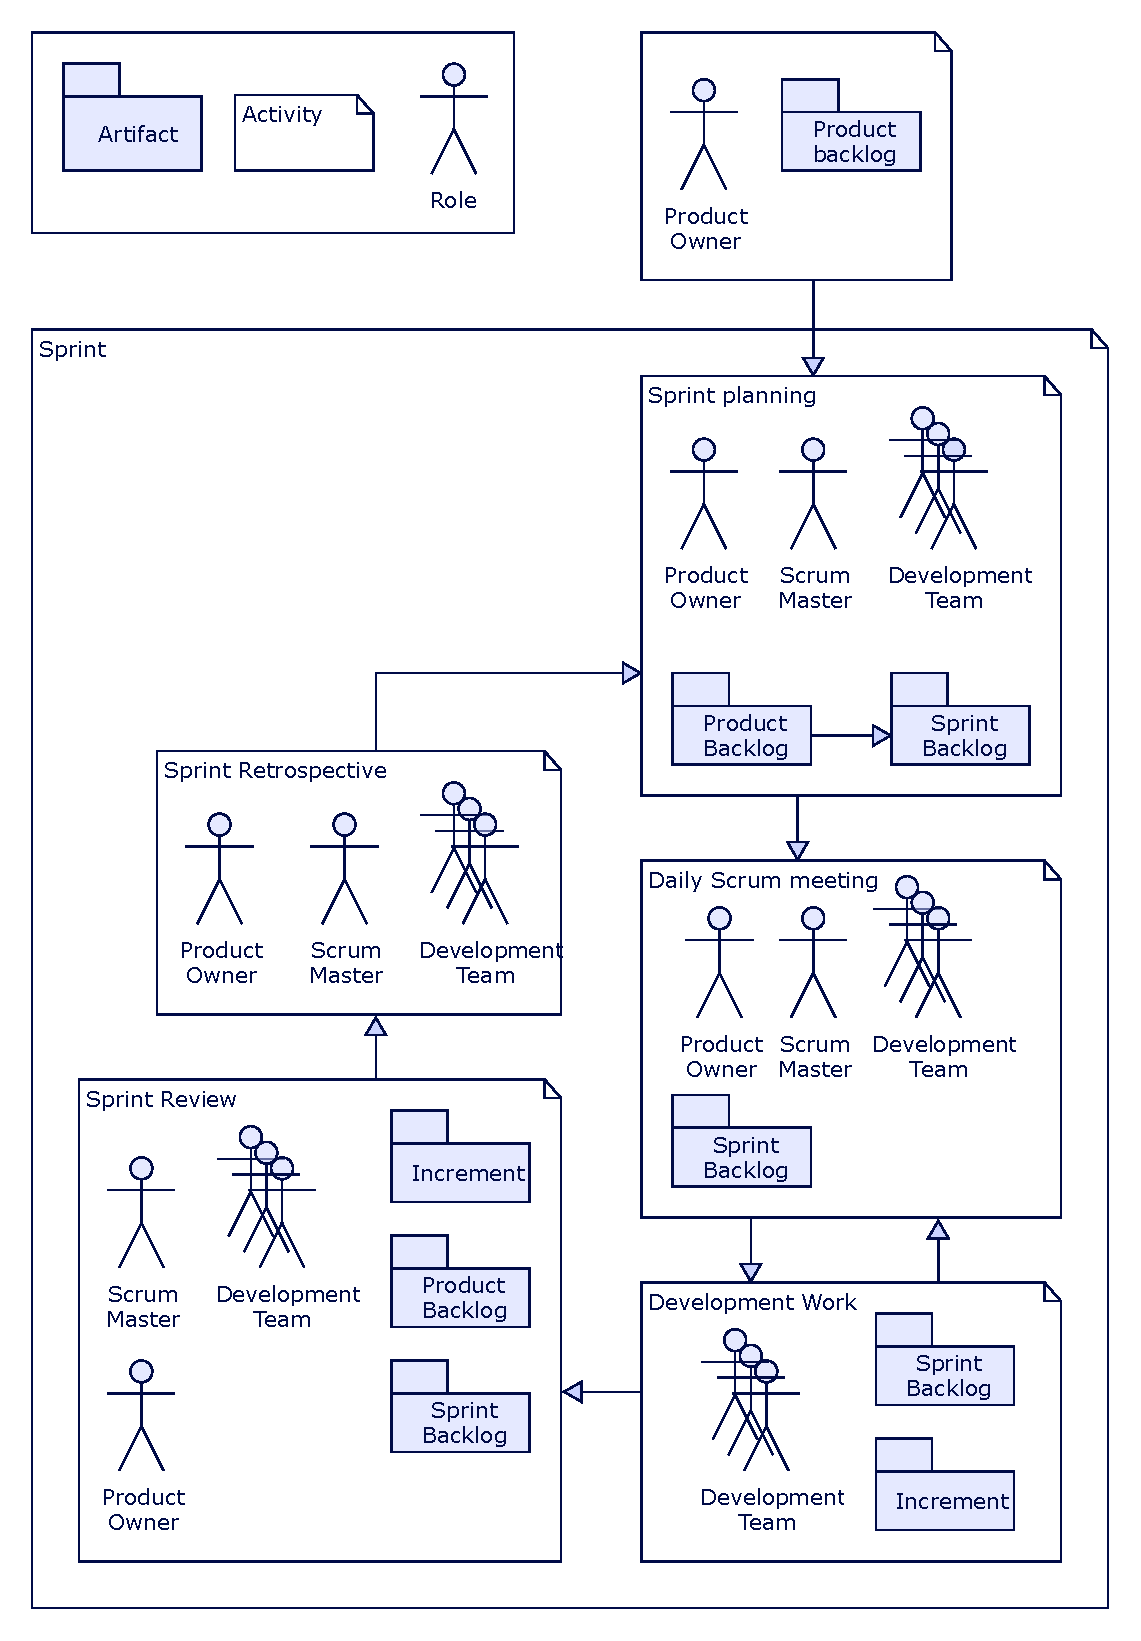
\includegraphics[scale=0.75]{Figures/Scrum_workflow.pdf}
	\decoRule
	\caption{The Scrum workflow.}
	\label{fig:ScrumWorkflow}
\end{figure}